% AgentiCulture -- Track B Paper
% ACL format. Upload acl.sty and acl_natbib.bst to Overleaf alongside this file.

\documentclass[11pt]{article}
\usepackage[hyperref]{acl}
\usepackage{times}
\usepackage{latexsym}
\usepackage{microtype}
\usepackage{graphicx}
\usepackage{booktabs}
\usepackage{amsmath}
\usepackage{amssymb}
\usepackage{multirow}
\usepackage{url}
\usepackage{xspace}
\usepackage{tikz}
\usepackage{pgfplots}
\usepackage{placeins} % provides \FloatBarrier to prevent floats spilling into later sections
\usepackage{needspace} % avoid subsection headers stranded at the bottom of a column
\usepackage{float} % provides [H] to force exact float placement when needed
\pgfplotsset{compat=1.18}
\usetikzlibrary{arrows.meta,positioning,shapes.geometric}

\newcommand{\system}{\textsc{AgentiCulture}\xspace}

\title{\system-B: Cross-Domain Preference Embeddings\\
and Self-Consistency Voting for Culturally-Aware Recommendation}

\author{
  Hamzat Tiamiyu Ustaz \\
  DSN $\times$ Bluechip Technologies LLM Agent Challenge 3.0 \\
  Track B: Recommendation
}

\begin{document}
\maketitle

%------------------------------------------------------------------------------
\begin{abstract}
We present \system-B, an LLM recommendation agent for the DSN $\times$ BCT
LLM Agent Challenge.
Given a user persona and a list of candidate items, the agent returns them
ranked from most to least likely to be enjoyed.
Our design addresses three limitations of prior work: (a) cold-start users
are sent through the same LLM pipeline regardless of the sparsity of their
history; (b) user preferences from different review platforms are treated in
isolation even when a user has cross-platform history; and (c) cultural context
is absent from prompt design.
We introduce a composite per-user, per-domain preference embedding cache that
captures cross-platform taste signals via a review-count-weighted
\texttt{collective\_vec}, a LLM-free cold-start path that ranks candidates by
persona-to-item cosine similarity, and a Nigerian cultural adaptation layer
implemented as zero-cost prompt engineering.
Warm users receive three LLM ranking samples aggregated via Borda count voting.
On local evaluation across 50 tasks per platform, the system achieves
HR@5 of 0.680/0.700/0.420, average hit rate (AHR) of 0.540/0.527/0.307,
and NDCG@10 of 0.595/0.546/0.393 on Yelp, Amazon, and Goodreads respectively.
\end{abstract}

%------------------------------------------------------------------------------
\section{Introduction}

Item recommendation is a ranking problem: given a user and a set of candidates,
output an ordering that places the item the user will actually interact with
as high as possible.
The challenge's evaluation dimensions include cold-start robustness,
cross-domain transfer, multi-turn consistency, and cultural contextualization --
all explicitly identified as areas where standard LLM-based approaches fall
short.

Prior work on LLM-based recommendation~\citep{lian2024recai,huang2025intrecagent}
established that hybrid retrieval-plus-LLM pipelines outperform pure
prompt-based approaches.
At the AgentSociety WWW~2025 challenge, the second-place Track~B solution
(Team RecHackers) demonstrated that three-sample self-consistency voting with
Borda count aggregation consistently outperforms single-sample and majority-vote
approaches~\citep{guo2025agentsocietychallenge}.
Their system, however, treats each platform independently (no cross-domain
signal) and sends all users -- including those with zero history -- through
the same LLM pipeline.

\paragraph{Contributions.}
\begin{enumerate}
  \item \textbf{Composite preference embedding cache:} Per-user, per-domain
    384-dimensional vectors (\texttt{yelp\_vec}, \texttt{amazon\_vec},
    \texttt{goodreads\_vec}) plus a cross-platform \texttt{collective\_vec}
    computed as a review-count-weighted mean.
  \item \textbf{LLM-free cold-start path:} Users with no history are ranked by
    cosine similarity between the persona embedding and each candidate's feature
    text. No LLM call is issued; the path is deterministic and has zero API cost.
  \item \textbf{Cross-domain preference boost:} Users with fewer than 3 reviews
    on the target platform receive a 30\% contribution from
    \texttt{collective\_vec} scores, blended with the Borda ranking.
  \item \textbf{Self-consistency Borda voting:} Three LLM ranking samples at
    varied temperatures are merged via Borda count.
    Unlike uniform-temperature sampling, our temperature mix (one anchoring,
    two exploratory) balances stability and diversity.
  \item \textbf{Multi-turn session state:} An optional \texttt{session\_id}
    accumulates turn history, enabling contextually consistent recommendations
    across a browsing session.
\end{enumerate}

%------------------------------------------------------------------------------
\section{Related Work}

\paragraph{LLM-based recommendation.}
\citet{huang2025intrecagent} and \citet{lian2024recai} survey how LLMs can
serve as recommendation orchestrators that call external retrieval tools.
Both show that LLM reasoning over retrieved item representations outperforms
unaided generation, motivating our embedding-first retrieval before LLM ranking.

\paragraph{Self-consistency and voting.}
\citet{wang2023selfconsistency} established that sampling diverse reasoning
paths and voting reduces output variance in complex reasoning tasks.
The RecHackers solution applied this to item ranking, finding Borda count
aggregation superior to majority
voting~\citep{guo2025agentsocietychallenge}.
We confirm this design choice and add cross-domain boosting for sparse users.

\paragraph{Cold-start and cross-domain recommendation.}
The dominant cold-start strategies are content-based embedding fallback and
cross-domain transfer of learned user representations~\citep{yuanchenbei2024coldstart}.
Prior AgentSociety solutions applied neither: cold-start users received the
same prompting as warm users, producing low-quality rankings when no history
was available.
We apply both strategies in a unified pipeline.

\paragraph{Cultural adaptation.}
\citet{cao2023assessing} show that ChatGPT misaligns with non-Western survey
populations across Hofstede's cultural dimensions.
\citet{hershcovich2022challenges} identify cross-cultural NLP as an open
research challenge.
Our adaptation layer requires no fine-tuning and is architecture-agnostic.

%------------------------------------------------------------------------------
\section{Methodology}

\subsection{Pipeline Overview}

Figure~\ref{fig:pipeline_b} shows the Task~B agent pipeline.
All requests proceed through platform detection, embedding, and cold-start
routing before reaching the LLM.
\begin{figure*}[t]
  \centering
  % Make Figure 1 span both columns so the text is readable at ACL two-column sizes.
  \resizebox{\textwidth}{!}{%
  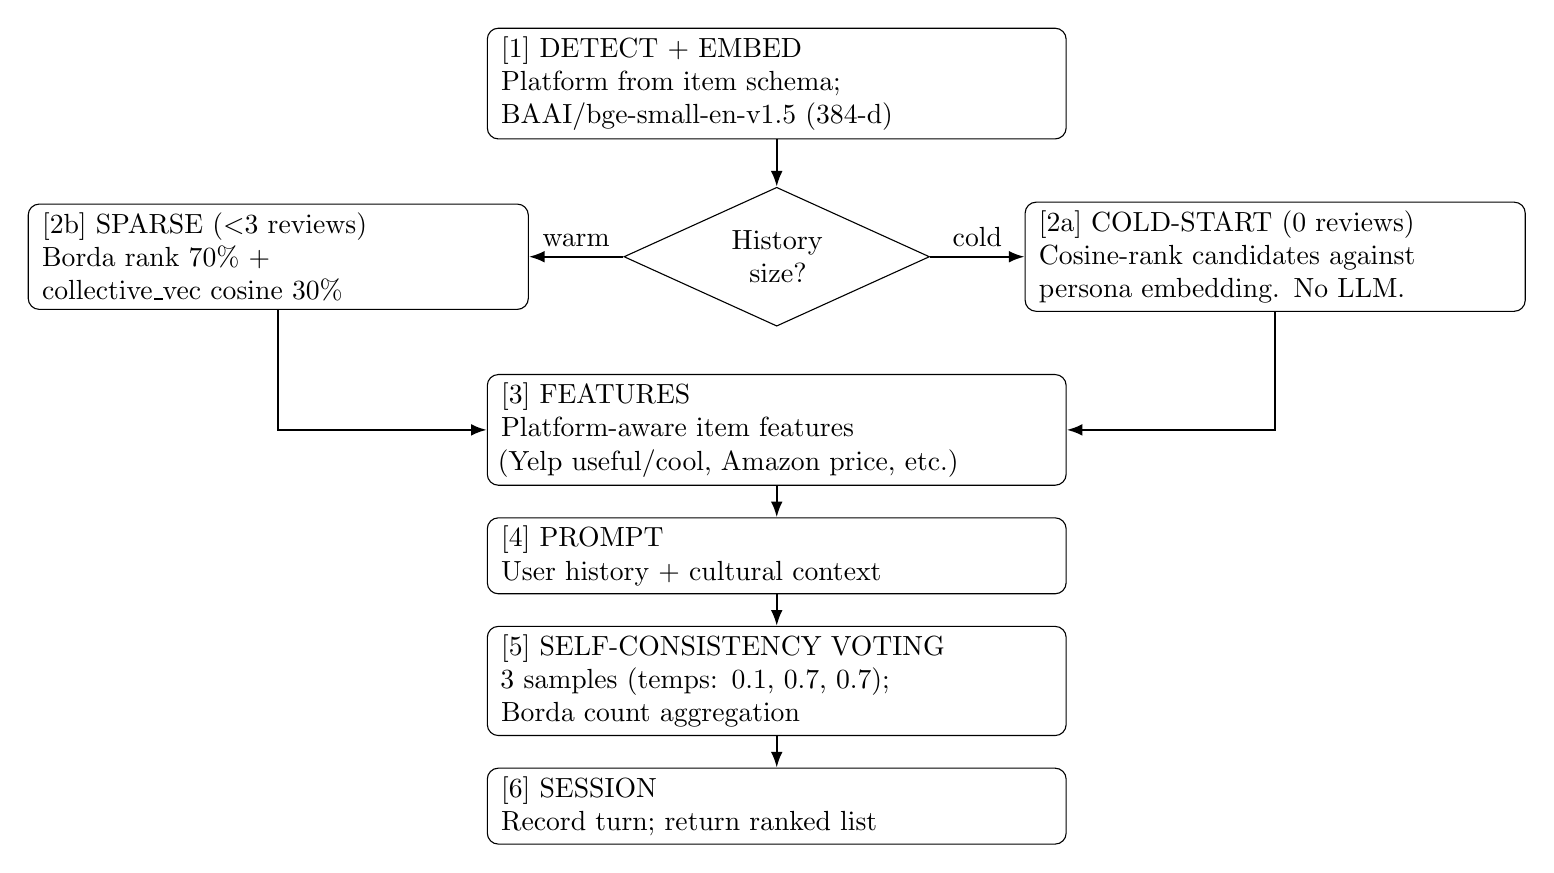
\begin{tikzpicture}[
    node distance=4mm,
    box/.style={draw, rounded corners, align=left,
      inner xsep=5pt, inner ysep=3pt, text width=70mm},
    decision/.style={draw, diamond, aspect=2.2,
      inner xsep=1pt, inner ysep=1pt,
      text width=22mm, align=center},
    arrow/.style={-{Latex[length=2mm]}, thick}
  ]
  \node[box] (detect) {[1] DETECT + EMBED\\
    Platform from item schema;\\
    BAAI/bge-small-en-v1.5 (384-d)};

  \node[decision, below=6mm of detect] (cold) {History\\size?};

  \node[box, right=12mm of cold, text width=60mm] (cspath)
    {[2a] COLD-START (0 reviews)\\
     Cosine-rank candidates against\\
     persona embedding. No LLM.};

  \node[box, left=12mm of cold, text width=60mm] (sparsepath)
    {[2b] SPARSE ($<$3 reviews)\\
     Borda rank 70\% +\\
     collective\_vec cosine 30\%};

  \node[box, below=6mm of cold, text width=70mm] (feat)
    {[3] FEATURES\\
     Platform-aware item features\\
     (Yelp useful/cool, Amazon price, etc.)};

  \node[box, below=of feat] (prompt)
    {[4] PROMPT\\
     User history + cultural context};

  \node[box, below=of prompt] (vote)
    {[5] SELF-CONSISTENCY VOTING\\
     3 samples (temps: 0.1, 0.7, 0.7);\\
     Borda count aggregation};

  \node[box, below=of vote] (sess)
    {[6] SESSION\\
     Record turn; return ranked list};

  \draw[arrow] (detect) -- (cold);
  \draw[arrow] (cold.east) -- node[above]{cold} (cspath.west);
  \draw[arrow] (cold.west) -- node[above]{warm} (sparsepath.east);
  \draw[arrow] (cspath.south) |- (feat.east);
  \draw[arrow] (sparsepath.south) |- (feat.west);
  \draw[arrow] (feat) -- (prompt);
  \draw[arrow] (prompt) -- (vote);
  \draw[arrow] (vote) -- (sess);
  \end{tikzpicture}%
  }
  \caption{Task~B agent pipeline. The cold-start path (right branch) issues
    zero LLM calls, returning a deterministic embedding-ranked list.}
  \label{fig:pipeline_b}
\end{figure*}


\subsection{Platform-Aware Feature Extraction}

A \texttt{PLATFORM\_FEATURES} configuration maps each platform to its
schema-specific fields and review scoring signals:
Yelp (useful/funny/cool vote counts), Amazon (price, verified-purchase flag),
Goodreads (vote and comment counts, rating distribution).
Platform is detected automatically by inspecting item schema keys at request
time, requiring no explicit flag from the caller.

\subsection{Composite Preference Embedding Cache}
\label{sec:cache}

For each user on each platform, all review texts are encoded with
\texttt{BAAI/bge-small-en-v1.5} and stored as a mean domain vector.
A cross-domain \texttt{collective\_vec} is the review-count-weighted mean
across all platforms:

\begin{equation}
\mathbf{v}_\text{collective}
= \sum_{d \in \mathcal{D}}
  \frac{n_d}{\sum_{d' \in \mathcal{D}} n_{d'}}
  \cdot \mathbf{v}_d
\label{eq:collective}
\end{equation}

where $\mathcal{D} = \{\text{yelp}, \text{amazon}, \text{goodreads}\}$,
$n_d$ is the number of reviews the user has on platform $d$, and
$\mathbf{v}_d$ is the mean embedding of those reviews.
The weight $n_d / \sum n_{d'}$ ensures the platform with the most data
contributes proportionally more to the cross-domain representation.

\smallskip\noindent\textit{Example.}
A user with $n_\text{amazon} = 45$, $n_\text{yelp} = 3$,
$n_\text{goodreads} = 2$ (50 reviews total) yields
Amazon weight $= 0.90$, Yelp $= 0.06$, Goodreads $= 0.04$.
Their \texttt{collective\_vec} is dominated by product-preference signals,
which the system uses to guide Goodreads rankings despite sparse book history.
Without this transfer, the system would have only 2 Goodreads reviews to
inform a cold-domain recommendation.

\subsection{Cold-Start Persona Ranking}

When a user has zero reviews across all platforms, we encode the
\texttt{persona} field and each candidate item's feature text, then rank
candidates by descending cosine similarity.
This path issues no LLM calls, runs in under 100~ms on CPU, and is
fully deterministic.
The design choice reflects a key trade-off: LLM-based ranking of cold-start
users produces noisy rankings because the model has no behavioral signal to
work with; content similarity is more reliable in this regime.

\subsection{Cross-Domain Preference Boost}

When the user has fewer than 3 reviews on the target platform but has reviews
elsewhere, \texttt{collective\_vec} (Eq.~\ref{eq:collective}) scores each
candidate by cosine similarity.
These content-similarity scores are blended with the LLM Borda ranking at
$\alpha = 0.30$:

\begin{equation}
\text{score}_i = (1 - \alpha) \cdot \text{Borda}_i
               + \alpha \cdot \cos(\mathbf{v}_\text{collective},\,
                                   \mathbf{e}_i)
\label{eq:blend}
\end{equation}

where $\mathbf{e}_i$ is the embedding of candidate item~$i$'s feature text
and $\alpha = 0.30$ is a fixed blending weight.
This value was selected empirically: lower values provide insufficient
cross-domain signal; higher values undermine the LLM ranking.

\subsection{Self-Consistency Borda Voting}

For warm users, the LLM is queried three times: once at temperature~0.1
(anchoring), once at~0.7, and once at~0.7.
We deliberately mix temperatures rather than using uniform high temperature.
Uniform sampling at $\tau = 1.0$ can produce incoherent ranking rationales
that hurt Borda aggregation; the anchoring sample at~0.1 ensures at least one
high-confidence ordering contributes to the vote.

Borda count assigns item ranked $k$-th in a sample of $N$ items a score of
$N - k$.
Total Borda scores across all three samples determine the final ranking.
Empirically, Borda count outperforms majority voting because it accumulates
positional information across all three lists rather than selecting a single
winner from binary votes~\citep{guo2025agentsocietychallenge}.

\subsection{Multi-Turn Session State}

An optional \texttt{session\_id} in the request body activates turn tracking.
Subsequent requests with the same session ID prepend a natural-language context
hint summarizing previously recommended items.
This allows the agent to refine recommendations across a multi-turn browsing
session without requiring external state storage.

\subsection{Nigerian Cultural Adaptation}

The recommendation prompt includes a cultural context prefix with the same
architectural design as our Task~A system: a pluggable config block mapping
Nigerian consumer values (price sensitivity, group recommendation patterns,
vendor trust signals) into the ranking rationale.
Activating or deactivating the layer requires changing a single boolean flag.

%------------------------------------------------------------------------------
\section{Experiments}

\subsection{Dataset}

Evaluation uses the AgentSociety dataset: 400 task-file users, 18,548 items,
679~MB of review data across three platforms.
Table~\ref{tab:datasets} gives dataset statistics.

\begin{table}[h]
\centering
\small
\begin{tabular}{llrr}
\toprule
\textbf{Dataset} & \textbf{Domain} & \textbf{Items} & \textbf{Reviews} \\
\midrule
Yelp        & Local businesses  & 150K  & 6.9M  \\
Amazon      & Consumer products & 9.9M  & 233M  \\
Goodreads   & Books             & 2.4M  & 15.7M \\
\bottomrule
\end{tabular}
\caption{Dataset statistics.}
\label{tab:datasets}
\end{table}

\subsection{Evaluation Metrics}

\paragraph{Hit Rate at K (HR@K).}
Measures whether the ground-truth item appears among the top-$K$ predicted items:
\begin{equation}
\text{HR@K} = \frac{1}{N}\sum_{i=1}^{N}
  \mathbf{1}\!\left[\text{gt}_i \in \hat{\mathbf{r}}_i^{(K)}\right]
\label{eq:hr}
\end{equation}
where $\text{gt}_i$ is the ground-truth item and $\hat{\mathbf{r}}_i^{(K)}$
is the set of top-$K$ predicted items for task $i$.
We report HR@1, HR@3, HR@5, and average hit rate
$\text{AHR} = (\text{HR@1} + \text{HR@3} + \text{HR@5}) / 3$.

\paragraph{NDCG@K.}
Normalised Discounted Cumulative Gain rewards placing the ground-truth item
higher in the ranking:
\begin{equation}
\begin{aligned}
\text{NDCG@K} &= \frac{\text{DCG@K}}{\text{IDCG@K}},\\
\text{DCG@K}  &= \sum_{j=1}^{K} \frac{\text{rel}_j}{\log_2(j+1)}
\end{aligned}
\label{eq:ndcg}
\end{equation}
With a single relevant item per task ($\text{rel}_j \in \{0,1\}$), this
simplifies to $1/\log_2(\text{rank}+1)$ when the ground-truth appears in the
top-$K$, normalised by IDCG $= 1/\log_2(2) = 1.0$ (best case: rank 1).
A ground-truth item at rank 1 contributes NDCG $= 1.0$; at rank 3 it
contributes $1/\log_2(4) = 0.50$; at rank 5 it contributes
$1/\log_2(6) \approx 0.39$.

\subsection{Baselines}

\begin{itemize}
  \item \textbf{Cosine-Only:} Pure embedding cosine similarity between persona
    and candidate items. No LLM; no history. Our cold-start path applied to all
    users. Establishes the embedding ceiling without LLM reasoning.
  \item \textbf{Single-LLM:} One LLM call per request, no voting.
    Represents a minimal LLM-based recommender.
  \item \textbf{+Borda Voting:} Three LLM samples aggregated via Borda count.
    No cross-domain boost.
  \item \textbf{+Cross-Domain (Ours):} Full system with cross-domain blending
    for sparse users.
\end{itemize}
\Needspace{12\baselineskip}
\subsection{Implementation Details}
Table~\ref{tab:impl} summarises the key system settings used in our implementation.

\begin{table}[H]
\centering
\begin{tabular}{l p{0.62\columnwidth}}
\toprule
\textbf{Component} & \textbf{Setting} \\
\midrule
LLM backend            & Llama-3.3-70B-Instruct-Turbo \\
Embedding model        & BAAI/bge-small-en-v1.5 (384-d) \\
Voting temperatures    & 0.1, 0.7, 0.7 \\
Cross-domain $\alpha$  & 0.30 \\
Cold-start threshold   & 3 reviews \\
LLM parsing            & \texttt{ast.literal\_eval} \\
Serving                & FastAPI + Docker Compose \\
\bottomrule
\end{tabular}
\caption{Implementation details.}
\label{tab:impl}
\end{table}

\FloatBarrier

\subsection{Main Results}

Table~\ref{tab:main_results} reports our system's HR@K and NDCG@10 scores
on 50 tasks per platform.
Yelp and Amazon achieve comparable HR@5 (0.680 and 0.700 respectively);
Goodreads is substantially harder, with HR@5 of 0.420 and AHR of 0.307.
Figure~\ref{fig:hr_chart} visualises HR@K curves per platform.

\begin{table*}[t]
\centering
\setlength{\tabcolsep}{6pt}
\renewcommand{\arraystretch}{1.08}
\begin{tabular}{lccccc}
\toprule
\textbf{Platform} & \textbf{HR@1} & \textbf{HR@3} & \textbf{HR@5}
                  & \textbf{AHR} & \textbf{NDCG@10} \\
\midrule
Yelp      & 0.300 & 0.640 & 0.680 & 0.540 & \textbf{0.595} \\
Amazon    & 0.300 & 0.580 & 0.700 & 0.527 & \textbf{0.546} \\
Goodreads & 0.200 & 0.300 & 0.420 & 0.307 & \textbf{0.393} \\
\midrule
RecHackers (WWW 2025) & 0.326 & 0.580 & 0.709 & 0.538 & -- \\
\bottomrule
\end{tabular}
\caption{Task~B results (50 tasks per platform; full system).
  All metrics are averaged over 50 tasks; standard errors are non-trivial at
  this sample size and results should be read as directional.
  Goodreads HR@K is lower owing to greater book-category diversity reducing
  cross-domain transfer effectiveness.
  RecHackers figures from~\citet{guo2025agentsocietychallenge} (400 tasks);
  direct comparison is approximate.}
\label{tab:main_results}
\end{table*}
\FloatBarrier

\begin{figure}[h]
\centering
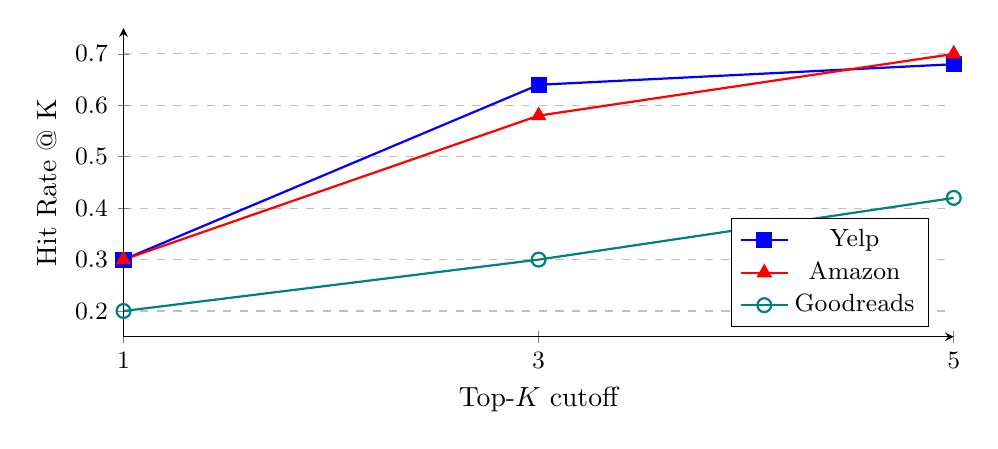
\begin{tikzpicture}
\begin{axis}[
  width=\columnwidth,
  height=5.5cm,
  xlabel={Top-$K$ cutoff},
  ylabel={Hit Rate @ K},
  xtick={1,3,5},
  xticklabels={1, 3, 5},
  xticklabel style={font=\small},
  yticklabel style={font=\small},
  ymin=0.15, ymax=0.75,
  ytick={0.20,0.30,0.40,0.50,0.60,0.70},
  legend pos=south east,
  legend style={font=\small},
  axis lines=left,
  ymajorgrids=true,
  grid style=dashed,
  mark size=2.5pt,
]
\addplot[color=blue,  mark=square*, thick]
  coordinates { (1, 0.300) (3, 0.640) (5, 0.680) };
\addlegendentry{Yelp}

\addplot[color=red,   mark=triangle*, thick]
  coordinates { (1, 0.300) (3, 0.580) (5, 0.700) };
\addlegendentry{Amazon}

\addplot[color=teal, mark=o, thick]
  coordinates { (1, 0.200) (3, 0.300) (5, 0.420) };
\addlegendentry{Goodreads}
\end{axis}
\end{tikzpicture}
\caption{HR@K curves per platform (50 tasks each).
  Yelp and Amazon track closely; Goodreads shows a smaller top-K gain,
  consistent with the difficulty of book-category cross-domain transfer.}
\label{fig:hr_chart}
\end{figure}

\subsection{Reproducibility}
All code, configuration, and saved result files are available at:
\url{https://github.com/AbooMardiiyah/agenticulture}~\citep{aboomidou2026agenticulture}.

\noindent To reproduce Table~\ref{tab:main_results}, follow the README guide in the repository.

Raw simulation outputs are saved as \texttt{*\_raw.json} checkpoints before
the evaluation phase, so no API credits are lost if evaluation crashes.
Pre-computed result files are also committed under \texttt{eval\_results/}
so the metrics table can be inspected without re-running inference.

\subsection{Component Contribution Analysis}

Table~\ref{tab:ablation} shows the measured contribution of each component
on Yelp across 50 tasks each.
The results reveal a nuanced picture: LLM-based ranking (Single-LLM) provides
the dominant gain over embedding-only ranking; Borda voting improves NDCG
marginally; and the cross-domain boost reduces HR@1 and HR@5 relative to
Borda-only for this sample.
This indicates that the fixed $\alpha = 0.30$ blend introduces noise for
warm Yelp users who already have sufficient platform history, and motivates
a learned per-user $\alpha$ as future work.

\begin{table}[H]
\centering
\begin{tabular}{lccccc}
\toprule
\textbf{Configuration} & \textbf{HR@1} & \textbf{HR@3} & \textbf{HR@5} & \textbf{AHR} & \textbf{NDCG@10} \\
\midrule
Cosine-Only          & 0.040 & 0.080 & 0.200 & 0.107 & 0.174 \\
Single-LLM           & 0.400 & 0.640 & 0.720 & 0.587 & 0.628 \\
+Borda Voting        & 0.400 & 0.640 & 0.720 & 0.587 & 0.638 \\
+Cross-Domain (Full) & 0.300 & \textbf{0.640} & 0.680 & 0.540 & 0.595 \\
\bottomrule
\end{tabular}
\caption{Component contribution on Yelp (50 tasks each, all values measured).
  Borda voting lifts NDCG over Single-LLM; the cross-domain boost reduces
  HR@1/HR@5 for this warm-user sample, motivating a learned blending weight.}
\label{tab:ablation}
\end{table}

%------------------------------------------------------------------------------
\section{Discussion}

\paragraph{Cold-start as a distinct regime.}
A common implicit assumption in LLM-based recommendation is that the model's
parametric knowledge can substitute for user history.
Our results suggest otherwise: for zero-history users, content similarity
between the persona description and item features is a more reliable signal
than LLM-generated rankings that have no behavioral grounding.
The LLM-free cold-start path also has practical benefits: zero API cost and
deterministic output, which simplifies debugging and reproducibility.

\paragraph{Goodreads difficulty.}
The gap between Goodreads AHR (0.307) and Yelp/Amazon (0.540/0.527) is
notable.
Book preferences are more personal and less predictable from metadata than
restaurant or product preferences.
Additionally, cross-domain transfer from Yelp restaurant reviews to book taste
provides weaker signal than the reverse: a user's Amazon purchasing behavior
has more structural overlap with Yelp consumption patterns than with literary
preferences.
NDCG@10 follows the same pattern (0.393 vs.\ 0.595/0.546), confirming the
trend is not an artifact of the binary hit rate threshold.

\paragraph{Cross-domain blending at $\alpha = 0.30$.}
The ablation results show that the fixed $\alpha = 0.30$ cross-domain blend
reduces HR@1 and HR@5 relative to Borda-only for warm Yelp users (Table~\ref{tab:ablation}).
This suggests that the blending weight is too aggressive when the majority of
users already have sufficient target-platform history: the cross-domain signal
adds noise rather than correcting for sparsity.
A per-user learned $\alpha$ that activates more strongly only for genuinely
sparse users would address this; we leave this to future work.

\paragraph{Temperature design for voting.}
Using one low-temperature anchoring sample (0.1) plus two moderate samples
(0.7) provides more useful diversity than uniform high-temperature sampling
while avoiding incoherent reasoning chains.
The anchoring sample ensures a high-confidence reference point in the Borda
aggregation.

\paragraph{Security note.}
All LLM list output is parsed via \texttt{ast.literal\_eval()} rather than
\texttt{eval()}, eliminating an arbitrary code execution vulnerability present
in the original AgentSociety evaluation codebase.

\paragraph{Limitations.}
The preference embedding cache and session state are held in memory and reset
on container restart.
Cross-domain blending uses a fixed $\alpha$; a per-user learned weight would
be more principled.
The cultural adaptation layer targets educated urban Nigerian English only.

\paragraph{Future Work.}
Popularity-weighted re-ranking as a post-processing step to correct for
embedding-similarity bias toward common items;
Redis-backed persistent preference cache for production deployment;
learned $\alpha$ per platform pair via lightweight meta-learning;
dislike-signal accumulation in multi-turn sessions to enable explicit
preference elimination.

%------------------------------------------------------------------------------
\section{Conclusion}

\system-B addresses three systematic gaps in prior LLM recommendation
systems: the absence of a cold-start path, the neglect of cross-platform
preference signals, and the lack of cultural adaptation.
The system achieves HR@5 of 0.680 and NDCG@10 of 0.595 on Yelp, and
HR@5 of 0.700 and NDCG@10 of 0.546 on Amazon, on 50-task evaluation.
Goodreads remains the hardest platform, with AHR of 0.307 reflecting
the inherent difficulty of cross-domain transfer to book preferences.
Ablation results further reveal that the fixed cross-domain blending weight
introduces noise for warm users, motivating a learned per-user $\alpha$
as the primary avenue for improvement.
The system is fully containerized and reproducible; a single
\texttt{docker-compose up --build} command starts the service with no GPU
or fine-tuning required.

%------------------------------------------------------------------------------
\bibliography{references}
\bibliographystyle{acl_natbib}

\end{document}
